%
% buchcover.tex -- Cover für das Buch Numerik
%
% (c) 2018 Prof Dr Andreas Müller, Hochschule Rapperswil
%
\documentclass[11pt]{standalone}
\usepackage{tikz}
\usepackage{times}
\usepackage{geometry}
\usepackage{german}
\usepackage[utf8]{inputenc}
\usepackage[T1]{fontenc}
\usepackage{times}
\usepackage{amsmath,amscd}
\usepackage{amssymb}
\usepackage{amsfonts}
\usepackage{txfonts}
\usepackage{ifthen}
\usepackage{qrcode}
\usetikzlibrary{math}
\geometry{papersize={402mm,278mm},total={405mm,278mm},top=72.27pt, bottom=0pt, left=72.27pt, right=0pt}
\newboolean{guidelines}
\setboolean{guidelines}{true}
\setboolean{guidelines}{false}

\begin{document}
\begin{tikzpicture}[>=latex, scale=1]
\tikzmath{
	real \ruecken, \einschlag, \gelenk, \breite, \hoehe;
	\ruecken = 3.0;
	\einschlag = 1.6;
	\gelenk = 0.8;
	\breite = 16.7;
	\hoehe = 24.6;
	real \bogengreite, \bogenhoehe;
	\bogenbreite = 2 * (\breite + \einschlag + \gelenk) + \ruecken;
	\bogenhoehe = 2 * \einschlag + \hoehe;
}

%\clip (0,0) circle (6);

\draw[fill=blue](0,0) rectangle({\bogenbreite},{\bogenhoehe});
\hsize=13.6cm

\begin{scope}
\clip (0,{0.0*\bogenhoehe}) rectangle({\bogenbreite},{0.6*\bogenhoehe});
%\clip (0,0) rectangle ({\bogenbreite},20.2);
%\node at (18.7,8.9) [scale=5.0]{\includegraphics{nozzle-hell.jpg}};
%\node at (18.7,8.9) [scale=5.0]{\includegraphics{nozzle-hell3.jpg}};
%\node at (18.7,8.9) [scale=5.0]{\includegraphics{nozzle.jpg}};
%\node at ({\bogenbreite/2},13.0) {\includegraphics[width=42cm]{matrix.pdf}};
\node at ({\bogenbreite/2+5},5.0) {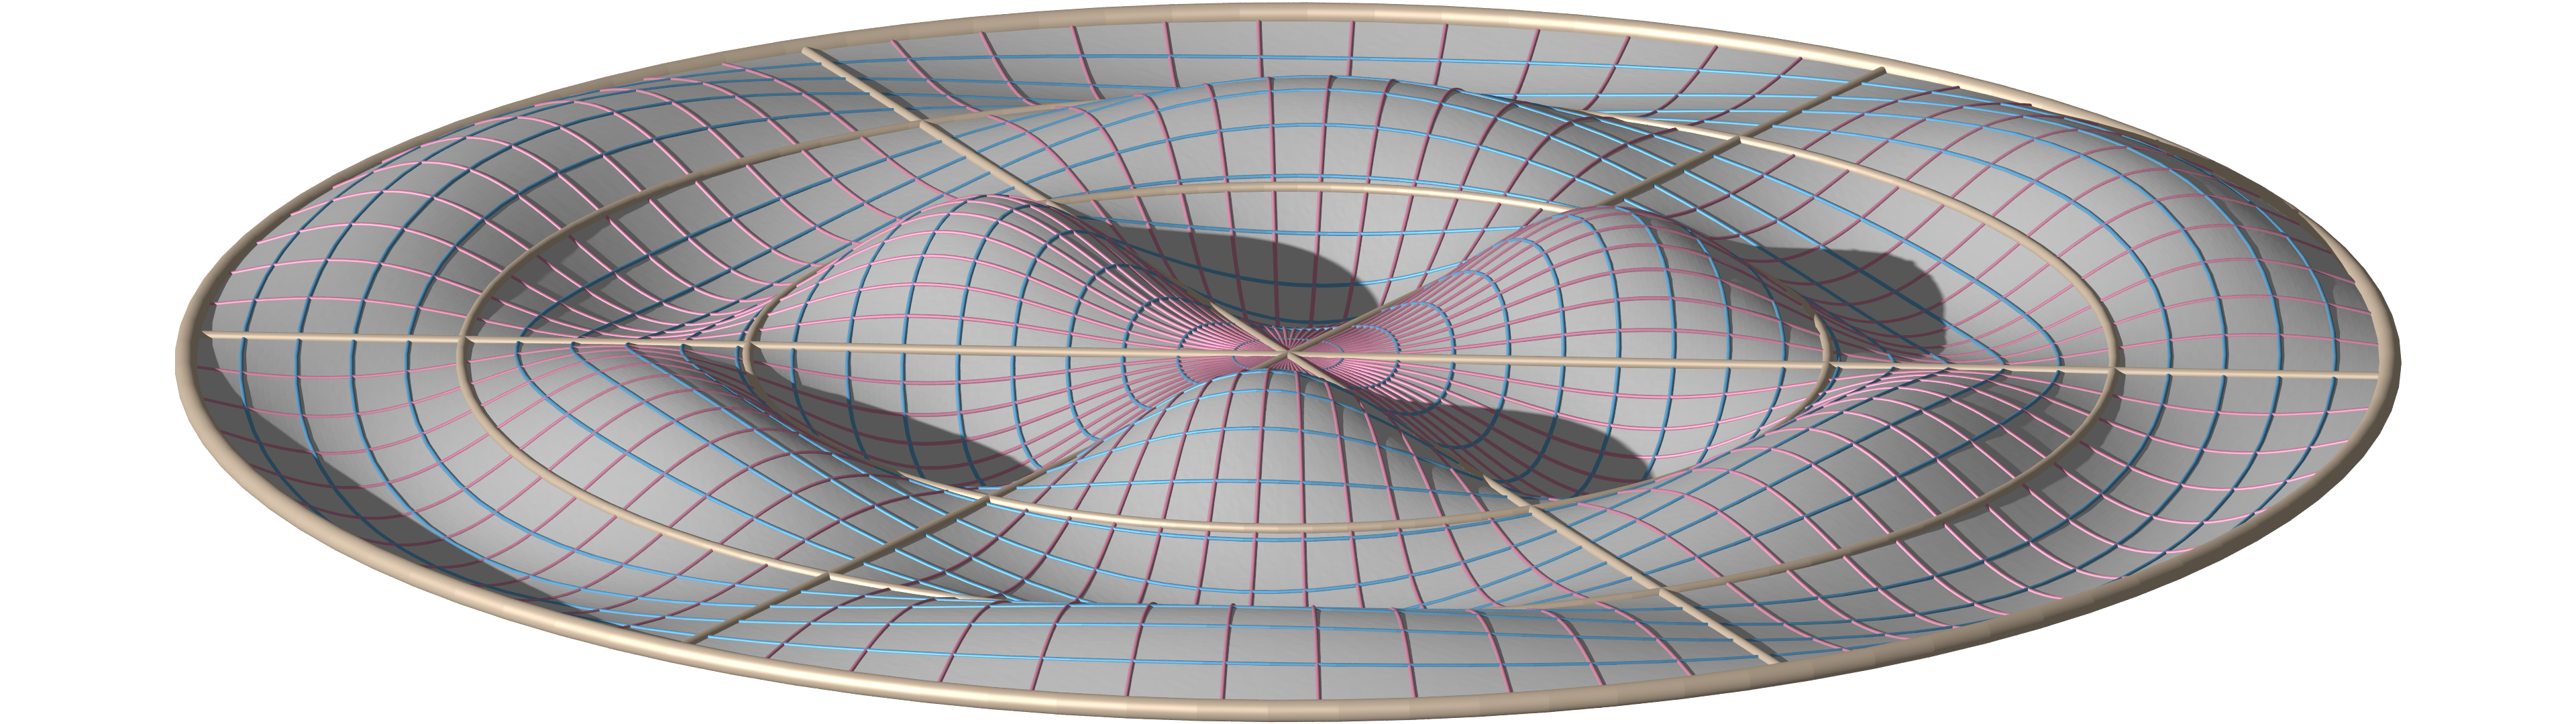
\includegraphics[width=42cm]{../buch/chapters/090-pde/membran/membran.png}};
\node at (11,11) {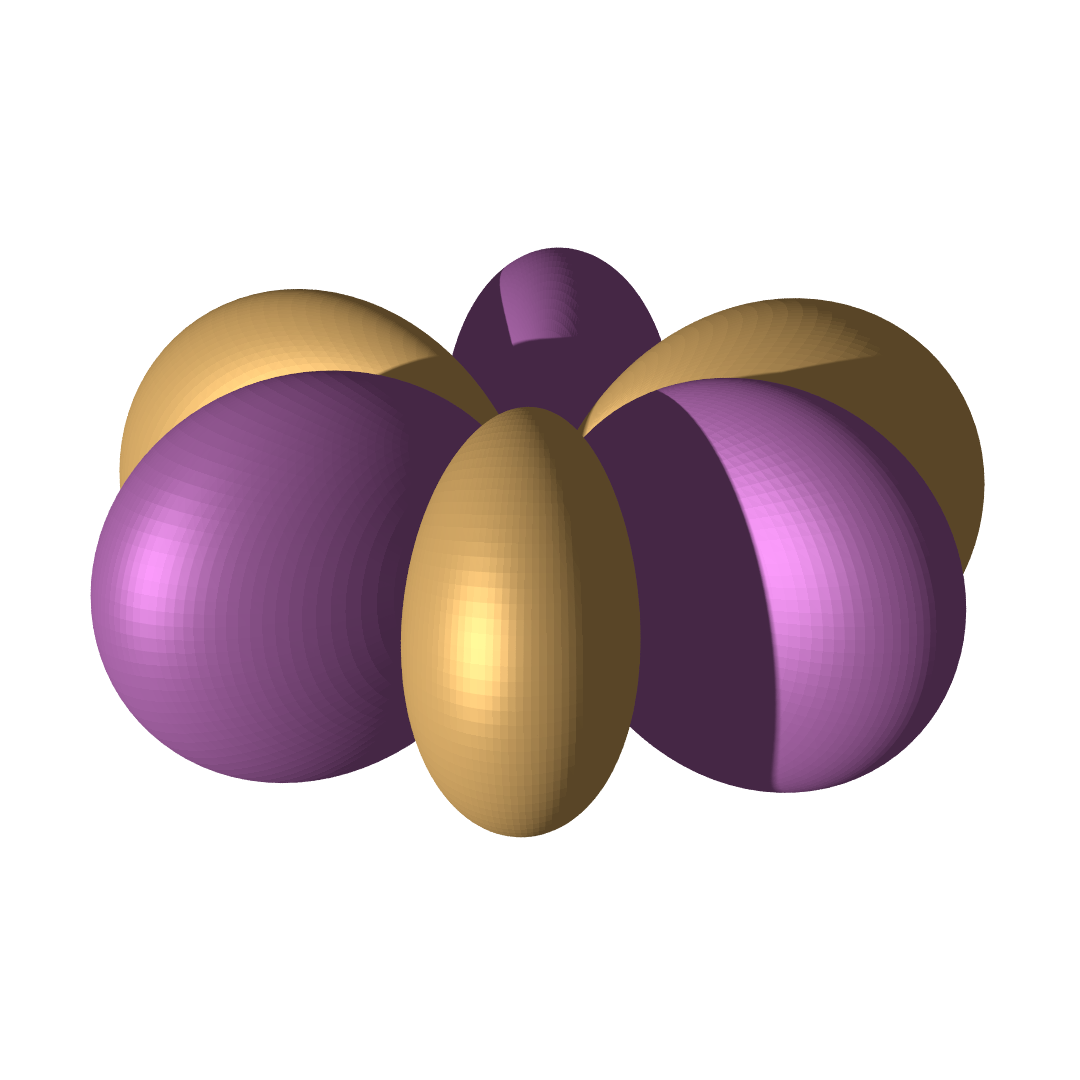
\includegraphics[width=8cm]{../buch/chapters/090-pde/kugel/spherical33.png}};
\node at (20,11) {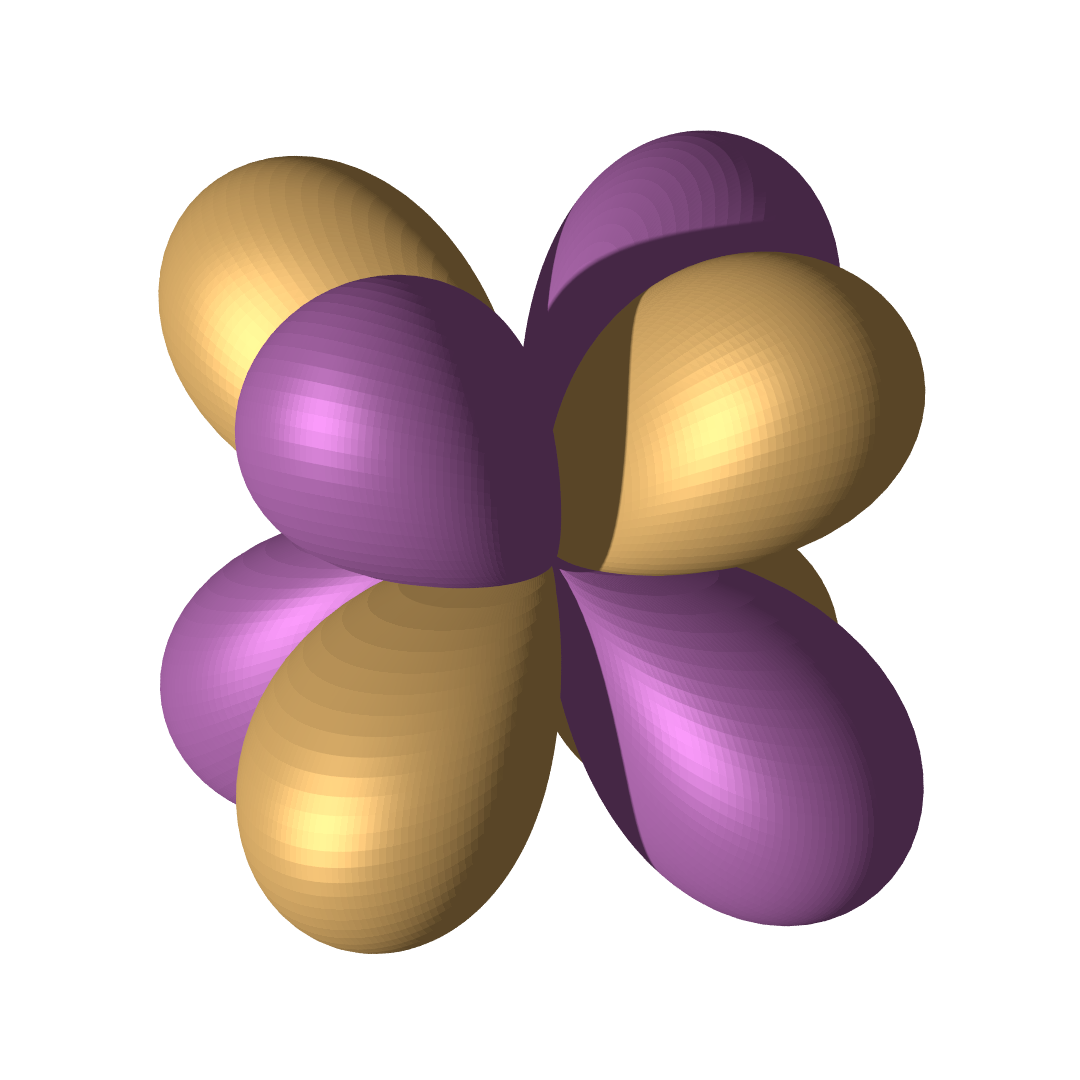
\includegraphics[width=8cm]{../buch/chapters/090-pde/kugel/spherical32.png}};
\node at (28,11) {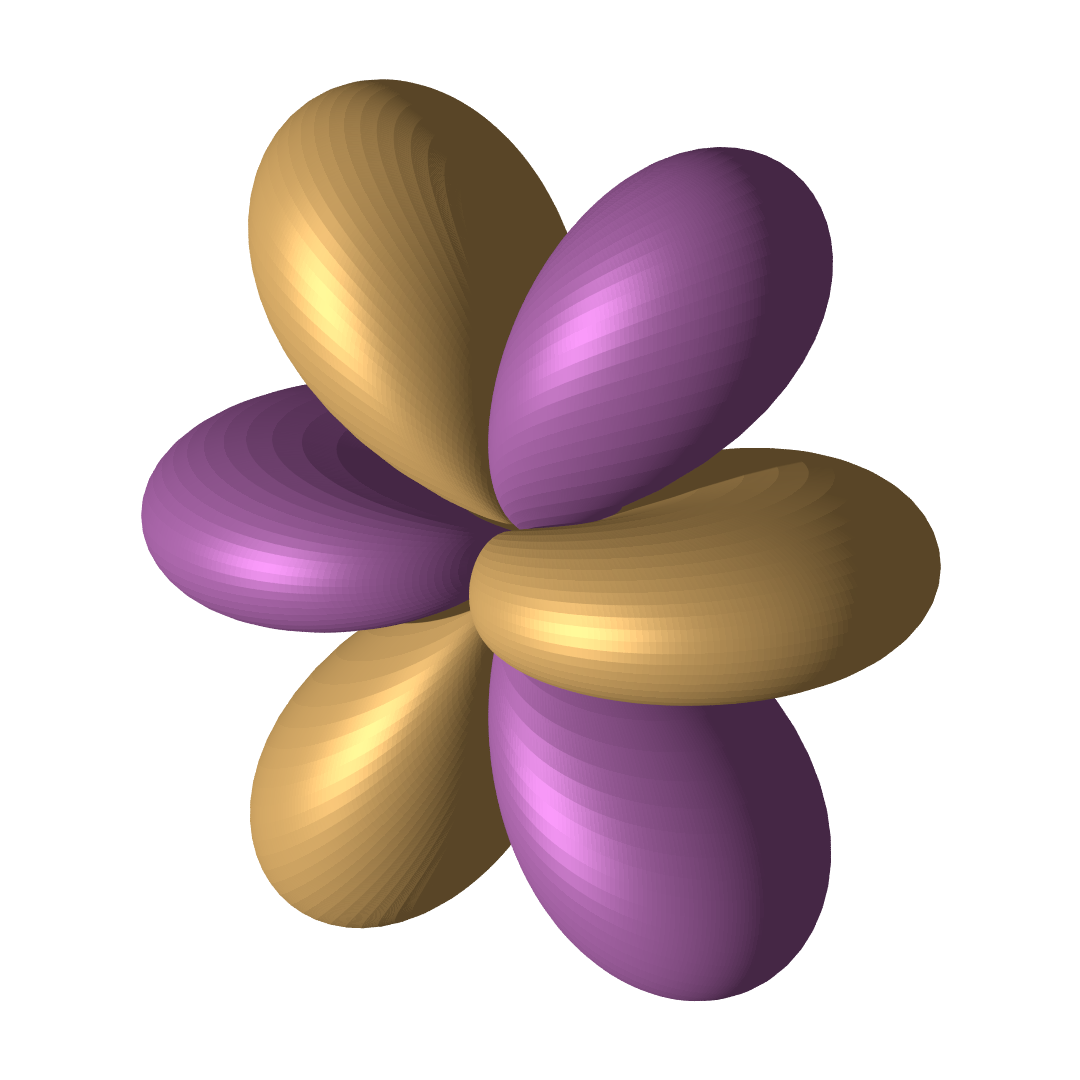
\includegraphics[width=8cm]{../buch/chapters/090-pde/kugel/spherical31.png}};
\node at (36,11) {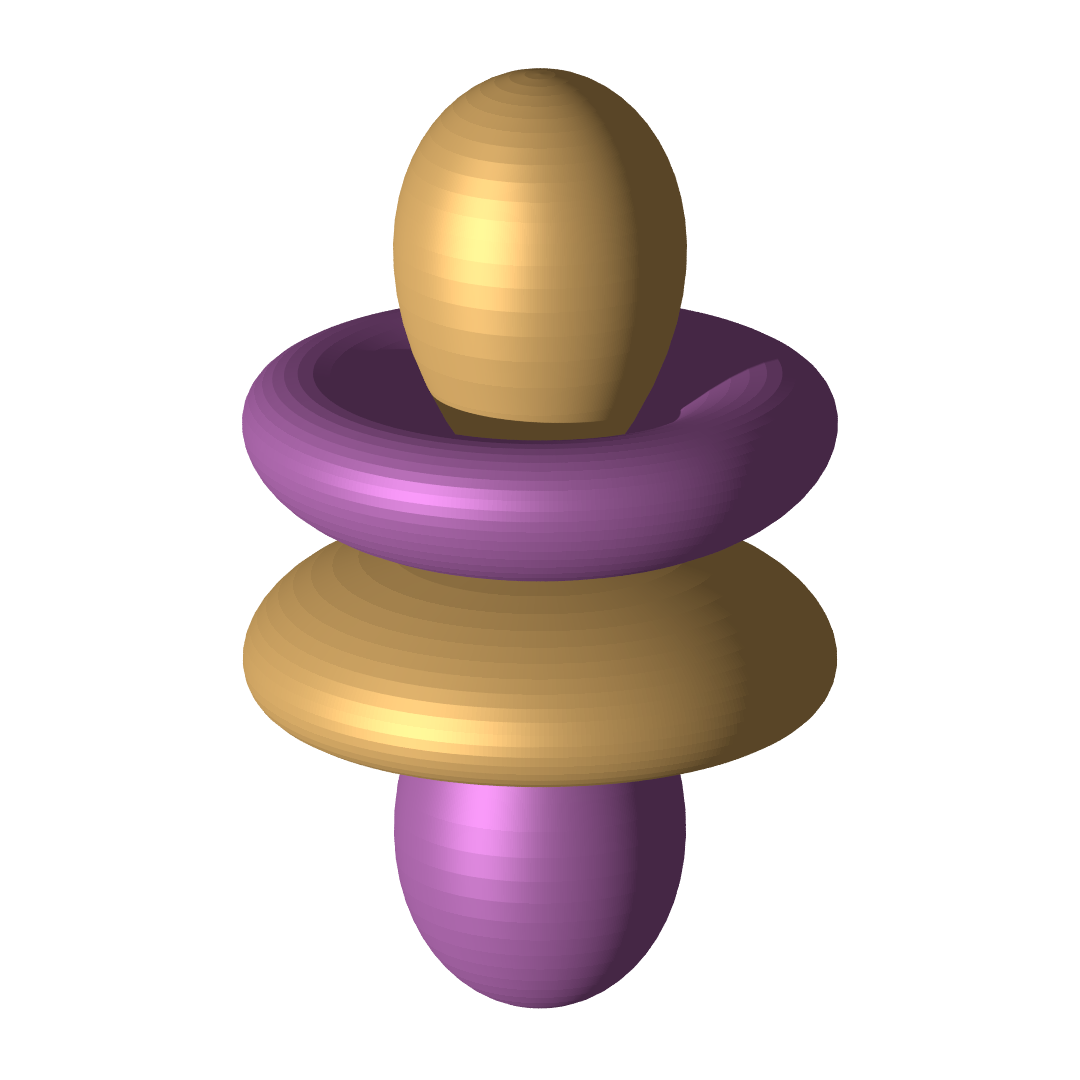
\includegraphics[width=8cm]{../buch/chapters/090-pde/kugel/spherical30.png}};
\end{scope}

\node at ({\einschlag+2*\gelenk+\ruecken+1.5*\breite},24.3)
	[color=white,scale=1]
	{\hbox to\hsize{\hfill%
	\sf \fontsize{24}{24}\selectfont Mathematisches Seminar}};

\node at ({\einschlag+2*\gelenk+\ruecken+1.5*\breite},21.9)
	[color=white,scale=1]
	{\hbox to\hsize{\hfill%
	\sf \fontsize{44}{44}\selectfont Spezielle Funktionen}};

\node at ({\einschlag+2*\gelenk+\ruecken+1.5*\breite},19.7)
	[color=white,scale=1]
	{\hbox to\hsize{\hfill%
	\sf \fontsize{13}{5}\selectfont Andreas Müller}};

\node at ({\einschlag+2*\gelenk+\ruecken+1.5*\breite},18.4)
	[color=white,scale=1]
	{\hbox to\hsize{\hfill%
	\sf \fontsize{13}{5}\selectfont
	Joshua Bär,                     % E
	Selvin Blöchlinger,		% E
	Marc Benz,			% MSE
	Manuel Cattaneo%,		% MSE
	}};

\node at ({\einschlag+2*\gelenk+\ruecken+1.5*\breite},17.75)
	[color=white,scale=1]
	{\hbox to\hsize{\hfill%
	\sf \fontsize{13}{5}\selectfont
	Fabian Dünki,                  % E
	Robin Eberle,                   % E
	Enez Erdem,                     % B
	Nilakshan Eswararajah%,          % B
	}};

\node at ({\einschlag+2*\gelenk+\ruecken+1.5*\breite},17.1)
	[color=white,scale=1]
	{\hbox to\hsize{\hfill%
	\sf \fontsize{13}{5}\selectfont
	Réda Hadouche,			% E
	David Hugentobler,              % E
	Alain Keller,                   % E
	Yanik Kuster%,                   % E
	}};
 
\node at ({\einschlag+2*\gelenk+\ruecken+1.5*\breite},16.45)
	[color=white,scale=1]
	{\hbox to\hsize{\hfill%
	\sf \fontsize{13}{5}\selectfont
	Marc Kühne,                    % B
	Erik Löffler,                   % E
	Kevin Meili,                    % M-I
	Andrea Mozzini Vellen%,          % E
	}};

\node at ({\einschlag+2*\gelenk+\ruecken+1.5*\breite},15.8)
	[color=white,scale=1]
	{\hbox to\hsize{\hfill%
	\sf \fontsize{13}{5}\selectfont
	Patrick Müller,                % MSE
	Naoki Pross,                    % E
	Thierry Schwaller,              % E
	Tim Tönz%                       % E
	%
	}};

\node at ({\einschlag+2*\gelenk+\ruecken+1.5*\breite},15.15)
	[color=white,scale=1]
	{\hbox to\hsize{\hfill%
	\sf \fontsize{13}{5}\selectfont
	%Reto Wildhaber%			% B
	}};
 
%\node at (0,3) [color=white] {\sf \LARGE Mathematisches Seminar 2017};

% Rücken
\node at ({\bogenbreite/2 + 0.00},18.5) [color=white,rotate=-90]
	{\sf\fontsize{35}{0}\selectfont Spezielle Funktionen\strut};

% Buchrückseite
\node at ({\einschlag+0.5*\breite},18.6) [color=white] {\sf
\fontsize{13}{16}\selectfont
\vbox{%
\parindent=0pt
%\raggedright
Das Mathematische Seminar der Ostschweizer Fachhochschule
in Rapperswil hat sich im Frühjahrssemester 2022 dem Thema
Spezielle Funktionen
zugewandt.
Ziel war, die grosse Vielfalt von speziellen Funktionen und
Funktionenfamilien zu ergründen, die im Laufe der Zeit für die
verschiedensten Anwendungen erdacht wurden.
Dieses Buch bringt das Skript des Vorlesungsteils mit den von den
Seminarteilnehmern beigetragenen Seminararbeiten zusammen.
}};

\def\qrbreite{3}
\def\qrrightoffset{0}
\def\qrbottomoffset{1.5}

\fill[color=white]
        ({\einschlag+(\breite+13.6)/2-\qrbreite-0.1},{\einschlag+\qrbottomoffset-0.1})
        rectangle
        ({\einschlag+(\breite+13.6)/2+0.1},{\einschlag+\qrbottomoffset+\qrbreite+0.1});

\node at ({\einschlag+(\breite+13.6)/2-\qrbreite/2},{\einschlag+\qrbottomoffset+\qrbreite/2}) {
\qrcode[height=3cm]{https://github.com/AndreasFMueller/SeminarSpezielleFunktionen/releases/download/v1.0.0/SeminarSpezielleFunktionen.pdf}
};
\node at ({\einschlag+(\breite+13.6)/2-\qrbreite/2},{\einschlag+\qrbottomoffset+\qrbreite/2}) {

\includegraphics[width=10mm]{mathman.png}
};

\ifthenelse{\boolean{guidelines}}{
\draw[white] (0,{\einschlag})--({\bogenbreite},{\einschlag});
\draw[white] (0,{\bogenhoehe-\einschlag})--({\bogenbreite},{\bogenhoehe-\einschlag});

\draw[white] ({\einschlag},0)--({\einschlag},{\bogenhoehe});
\draw[white] ({\einschlag+\breite},0)--({\einschlag+\breite},{\bogenhoehe});
\draw[white] ({\einschlag+\breite+\gelenk},0)--({\einschlag+\breite+\gelenk},{\bogenhoehe});
\draw[white] ({\bogenbreite-\einschlag-\breite-\gelenk},0)--({\bogenbreite-\einschlag-\breite-\gelenk},{\bogenhoehe});
\draw[white] ({\bogenbreite-\einschlag-\breite},0)--({\bogenbreite-\einschlag-\breite},{\bogenhoehe});
\draw[white] ({\bogenbreite-\einschlag},0)--({\bogenbreite-\einschlag},{\bogenhoehe});
}{}

\end{tikzpicture}
\end{document}
